%% IEEE Conference Paper — Pixels to Steps
%% Compatible with Overleaf (pdflatex)
\documentclass[conference]{IEEEtran}

% ── Packages ──────────────────────────────────────────────────────────────────
\usepackage[T1]{fontenc}
\usepackage[utf8]{inputenc}
\usepackage{amsmath,amssymb,bm}
\usepackage{graphicx}
\usepackage{booktabs}
\usepackage{cite}
\usepackage{url}
\usepackage{hyperref}
\usepackage{tikz}
\usetikzlibrary{arrows.meta,positioning,shapes.geometric,calc,fit,backgrounds,
                decorations.pathreplacing}
\usepackage{subcaption}
\usepackage{xcolor}
\usepackage{microtype}

% ── Macros ────────────────────────────────────────────────────────────────────
\newcommand{\bx}{\bm{x}}
\newcommand{\bu}{\bm{u}}
\newcommand{\by}{\bm{y}}
\newcommand{\bxhat}{\hat{\bm{x}}}
\newcommand{\AL}{A_L}
\newcommand{\BL}{B_L}
\newcommand{\Lmat}{\bm{L}}
\newcommand{\Kmat}{\bm{K}}
\newcommand{\R}{\mathbb{R}}

% ─────────────────────────────────────────────────────────────────────────────
\title{Data-Efficient Linear Visual State Estimation}

\author{%
  \IEEEauthorblockN{Karthik Shivashankaran}
  \IEEEauthorblockA{
    New York University, New York, USA
  }
}

% ─────────────────────────────────────────────────────────────────────────────
\begin{document}
\maketitle

\begin{abstract}
Lee \emph{et al.}~\cite{lee2024} demonstrate that a pixel-based Luenberger
observer whose gain matrix is learned from teacher demonstrations via linear
least squares can achieve reliable cartpole stabilisation using only a
robot-facing camera---a method they call \emph{pixels to torques}.
This work implements and evaluates a closely related hybrid observer in
simulation.  The observer combines nominal linearised dynamics with a Ridge
regression model that maps raw binary pixel frames to pole-angle estimates,
which are blended into the model prediction.  Trained on 150 teacher
demonstrations and evaluated on 100 random initial conditions under true plant
mismatch, the observer achieves \textbf{100\% survival} and \textbf{79\%
paper-success} (cart $\leq0.176$~m, pole $\leq2^\circ$ at $t=2.5$~s).
The paper discusses how this simplified single-state-correction variant relates
to the full observer of Lee~\emph{et al.}~\cite{lee2024} and identifies
cart-position estimation as the primary remaining limitation.
\end{abstract}

% ─────────────────────────────────────────────────────────────────────────────
\section{Introduction}
\label{sec:intro}

A robotic arm operating in an unstructured environment has no intrinsic
knowledge of where objects are relative to its end-effector.  A camera is
therefore not optional: it is a fundamental requirement for any manipulation
task.  Given that the camera is already present, a natural question arises:
rather than building a layered perception pipeline to extract features, estimate
poses, and feed a separate controller, why not learn to map directly from pixels
to motor commands?

Existing approaches to vision-based control each carry significant limitations.
\textbf{Reinforcement learning (RL)} policies can handle rich dynamics but
require high-fidelity simulation to generate training data.  The resulting
sim-to-real gap degrades real-world performance, and closing it through domain
randomisation leaves policy performance on the
table~\cite{andrychowicz2020learning}.  \textbf{End-to-end vision-based RL}
removes the perception module entirely by learning a neural-network policy from
pixels to actions.  However, it demands orders of magnitude more data than
model-based methods, and the resulting network is often too compute-intensive to
run at the high control frequencies required for dynamic
tasks~\cite{levine2016end}.

\textbf{Linear vision-based control}~\cite{lee2024} resolves both limitations.
A Luenberger observer~\cite{luenberger1964} is learned directly on hardware via
linear regression, using demonstration data from a privileged teacher controller
with access to ground-truth sensor readings.  The result is a policy that trains
in minutes, requires as few as 20 demonstrations, achieves a 97\% stabilisation
success rate with 40 training trajectories and 100\% with 80~\cite{lee2024}, and
runs as a single matrix multiply at inference time with no GPU and no simulator.

As a first step toward extending this framework to multi-axis systems, this work
considers a cartpole mounted on a linear axis driven by a stepper motor.  This
platform preserves the key challenge of vision-only feedback while introducing a
control output that is a discrete step command $u_k\in\mathbb{Z}$ rather than a
continuous torque.  Stepper-driven linear axes are the building blocks of
low-cost robot arms, making the cartpole a natural stepping stone toward the
broader goal of pixels-to-steps control for multi-axis systems.  The present
study evaluates the observer in simulation using the Gymnasium
environment~\cite{brockman2016openai} as a testbed, with the application
scenario shown in Fig.~\ref{fig:scenario}.

% ─────────────────────────────────────────────────────────────────────────────
\section{Problem Definition}
\label{sec:problem}

\subsection{State Variables and Measurements}

Following the notation of Lee~\emph{et al.}~\cite{lee2024}, the discrete-time
cartpole state at time step~$k$ is
\begin{equation}
  \bx_k = \begin{bmatrix}
    x_k & \dot{x}_k & \theta_k & \dot{\theta}_k
  \end{bmatrix}^\top \in \R^4,
  \label{eq:state}
\end{equation}
where $x$~[m] is the signed horizontal cart displacement from the track
centre, $\dot{x}$~[m/s] the cart velocity, $\theta$~[rad] the pole angle
from the upright vertical (positive counter-clockwise), and
$\dot{\theta}$~[rad/s] the pole angular rate.

The sole sensor measurement is a binary grayscale camera frame
\begin{equation}
  \by^p_k \in \{0,255\}^{W\times H},
  \quad W = 600,\;H = 117\;\text{px},
\end{equation}
captured at 60~Hz.  Frames are binarised (pole pixels white on black
background) and zero-padded to a canonical $117\!\times\!600$ geometry.  The
control input $u_k\in\R$ is known because it is commanded by the controller.
The key geometric relationship exploited by the pixel-based observer is that the
pole-tip pixel column $u^*$ satisfies, to first order,
\begin{equation}
  u^* \approx \frac{W}{2\,x_{\max}}\,x + \frac{W\,l}{2\,x_{\max}}\,\theta,
  \label{eq:geometry}
\end{equation}
making the raw pixel vector an approximately linear function of
$(x,\theta)$---the geometric basis for the LLS approach of \cite{lee2024}.

\begin{figure}[t]
  \centering
  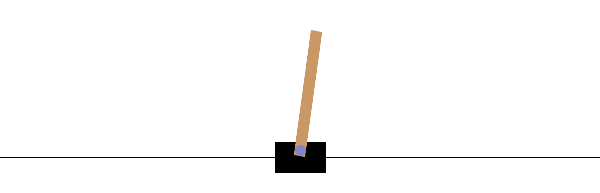
\includegraphics[width=0.85\columnwidth]{figures/gym_rgb_theta_+8deg_crop.png}\\[2pt]
  
\includegraphics[width=0.85\columnwidth]{figures/binary_theta_p08deg.png}
  \caption{\emph{Top:} simulation frame at $\theta_0 = +8^\circ$.
    \emph{Bottom:} corresponding binarised, zero-padded
    $117\!\times\!600$\,px observation~$\by^p$ supplied to the observer.
    The pole silhouette is the sole sensor signal; no encoder or IMU is
    available.}
  \label{fig:scenario}
\end{figure}

\subsection{Control Objective}

An LQR state-feedback gain $\Kmat\in\R^{1\times4}$ is designed on nominal plant
parameters.  The controller is
\begin{equation}
  u_k = -\Kmat\,\bxhat_k,
  \quad \Kmat = \begin{bmatrix}
    -31.5 & -79.8 & -970.8 & -109.5
  \end{bmatrix},
  \label{eq:lqr}
\end{equation}
where $\bxhat_k$ is the observer estimate.  The observer's task is to produce
estimates accurate enough for \eqref{eq:lqr} to stabilise the pole.

% ─────────────────────────────────────────────────────────────────────────────
\section{Data and Data Source}
\label{sec:data}

\subsection{Simulation Environment}

All data are collected in the Gymnasium CartPole-v1 environment~%
\cite{brockman2016openai}.  Nominal plant parameters are $m_c=1.0$~kg,
$m_p=0.1$~kg, $l=0.5$~m, $g=9.8$~m/s$^2$, $\tau=\tfrac{1}{60}$~s, and
actuator saturation $|u|\le10$~N.

To assess robustness, all evaluation rollouts use a mismatched true plant:
$m_p \leftarrow 1.1\,m_p$ and $l \leftarrow 0.9\,l$, mimicking the 5\%
parametric error used in~\cite{lee2024}.  The observer is unaware of the
mismatch.

\subsection{Teacher Demonstrations}

A privileged LQR teacher---with access to the full true state---collects
stabilising trajectories.  Following the protocol of Lee~\emph{et
al.}~\cite{lee2024}, each demonstration begins at rest ($x_0 = \dot x_0 =
\dot\theta_0 = 0$) with a fixed initial pole angle
$\theta_0\in\{\pm0.5^\circ,\pm1.0^\circ,\ldots,\pm12.0^\circ\}$, giving 150
unique trajectories each running for 150 steps (2.5~s at 60~Hz).

Frames are rendered at native resolution and zero-padded (top and symmetric
sides) to a canonical $117\!\times\!600$~px geometry.  Each frame is binarised
by thresholding to isolate the pole silhouette.  The resulting dataset contains
\textbf{35{,}928} (frame, state) pairs.  Fig.~\ref{fig:data} shows example
binarised frames across the angle range.

\begin{figure}[t]
  \centering
  
\includegraphics[width=0.95\columnwidth]{figures/binary_theta_m10deg.png}\\[-1pt]
  {\small$\theta_0 = -10^\circ$}\\[4pt]
  
\includegraphics[width=0.95\columnwidth]{figures/binary_theta_p00deg.png}\\[-1pt]
  {\small$\theta_0 = \phantom{+}0^\circ$}\\[4pt]
  
\includegraphics[width=0.95\columnwidth]{figures/binary_theta_p10deg.png}\\[-1pt]
  {\small$\theta_0 = +10^\circ$}
  \caption{Binarised $117\!\times\!600$\,px training frames at three initial
    angles.  The pole silhouette shifts laterally and tilts as $x$ and $\theta$
    change, providing the approximately linear pixel signal exploited by the
    Ridge regressor.}
  \label{fig:data}
\end{figure}

\subsection{Ridge Regression Fit Quality}

A Ridge regressor ($\alpha=0.1$) trained on the 150-demo dataset to predict
pole angle from the flattened pixel vector yields $R^2=0.986$,
RMSE~$=0.115^\circ$.  Only 12{,}952 of the 70{,}200 pixel coefficients are
nonzero, confirming the sparse spatial support concentrated on the pole-tip
region observed by Lee~\emph{et al.}~\cite{lee2024} in their Fig.~4.

% ─────────────────────────────────────────────────────────────────────────────
\section{Method of State Estimation}
\label{sec:method}

\subsection{Pixel-Based Luenberger Observer (Lee et al.)}

Lee~\emph{et al.}~\cite{lee2024} parameterise the observer as
\begin{equation}
  \bxhat_{k+1} = \AL\,\bxhat_k + \BL\,u_k + \Lmat\,\by^p_{k+1} + \bm{d},
  \label{eq:obs_lee}
\end{equation}
where $\AL\in\R^{4\times4}$, $\BL\in\R^{4\times1}$,
$\Lmat\in\R^{4\times WH}$, and $\bm{d}\in\R^4$ are all \emph{learned}
jointly.  Defining the parameter matrix
$\bm{\Theta}=[\AL,\BL,\Lmat,\bm{d}]$, teacher demonstration data are gathered
into matrices $\hat{X}_{2:N}$ (predicted next states) and $\Phi$ (current
states, inputs, pixel frames, bias column), then the regularised LLS problem is
solved:
\begin{equation}
  \min_{\bm{\Theta}}\;
  \|\bm{\Theta}\Phi - \hat{X}_{2:N}\|_F^2
  + \lambda\|\Lmat\|_1,
  \label{eq:lls}
\end{equation}
with an optional LMI constraint enforcing closed-loop stability.  Crucially,
\emph{all four rows} of $\Lmat$ are non-zero after fitting, meaning the
observer extracts pixel information relevant to $x$, $\dot x$, $\theta$, and
$\dot\theta$ simultaneously.

\subsection{Hybrid Observer (This Work)}

The implementation here fixes $\AL$, $\BL$ to the nominal linearised dynamics
(not learned) and sets $\Lmat=\bm{0}$, $\bm{d}=\bm{0}$.  Instead of
solving \eqref{eq:lls}, a Ridge regression model is trained separately to map
pixels to pole angle:
\begin{equation}
  \hat\theta^{\mathrm{px}}_{k+1}
  = \bm{c}_\theta^\top\,\bar{\by}^p_{k+1} + b_\theta,
  \label{eq:ridge}
\end{equation}
where $\bar{\by}^p\in[0,1]^{WH}$ is the normalised pixel vector.  The
predictor step is
\begin{equation}
  \bxhat^-_{k+1} = \AL\,\bxhat_k + \BL\,u_k,
  \label{eq:predict}
\end{equation}
and the angle component is corrected via a convex blend:
\begin{equation}
  \bxhat_{k+1}[2] \leftarrow
  (1-w_\theta)\,\bxhat^-_{k+1}[2]
  + w_\theta\,\hat\theta^{\mathrm{px}}_{k+1},
  \quad w_\theta = 0.7.
  \label{eq:blend}
\end{equation}
The remaining components ($x$, $\dot x$, $\dot\theta$) retain the model
prediction.  This is equivalent to \eqref{eq:obs_lee} with
\begin{equation}
  \Lmat_{\mathrm{eff}}[i,:] = \begin{cases}
    w_\theta\,\bm{c}_\theta^\top & i=2\;(\theta), \\
    \bm{0}^\top & \text{otherwise.}
  \end{cases}
  \label{eq:Leff}
\end{equation}

\subsection{Comparison to Prior Work}

Table~\ref{tab:compare} contrasts the hybrid observer against the full
learned observer of Lee~\emph{et al.}~\cite{lee2024}.

\begin{table}[t]
  \centering
  \caption{Observer Design Comparison}
  \label{tab:compare}
  \renewcommand{\arraystretch}{1.15}
  \begin{tabular}{lcc}
    \toprule
     & Lee et al.~\cite{lee2024} & This work \\
    \midrule
    $\AL,\BL$ & Learned (LLS) & Fixed (linearised) \\
    $\Lmat$ & Learned, all rows & Effective (1 row) \\
    $\bm{d}$ & Learned & Zero \\
    Training & Joint LLS & Separate Ridge \\
    Stability constraint & LMI (optional) & N/A \\
    States corrected & All 4 & $\theta$ only \\
    \bottomrule
  \end{tabular}
\end{table}

Unlike a Kalman filter, neither observer computes an error covariance or updates
the gain online.  The blend weight $w_\theta$ plays the role of a fixed Kalman
gain for the angle channel.  Compared to a particle filter, no Monte Carlo
sampling is required; the entire update is a single matrix-vector
product~\eqref{eq:predict} and one dot product~\eqref{eq:ridge}.

\subsection{System Block Diagram}

\begin{figure}[t]
  \centering
  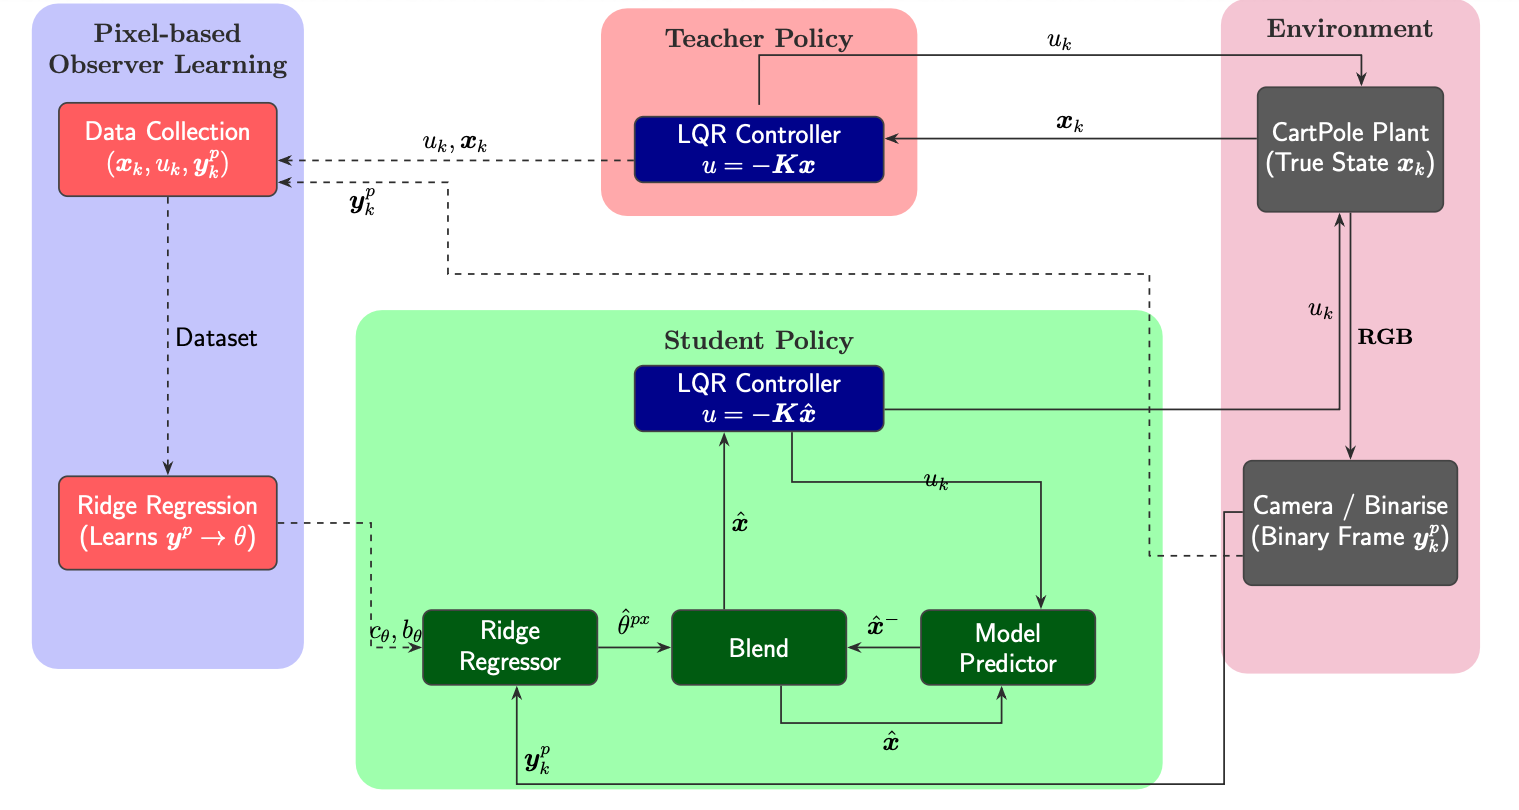
\includegraphics[width=\columnwidth]{figures/block.png}
  \caption{System block diagram. All signals are updated at 60~Hz.}
  \label{fig:blockdiagram}
\end{figure}

Fig.~\ref{fig:blockdiagram} shows the full signal flow.  At each 60~Hz
timestep: (1) the camera image is binarised; (2) the Ridge model produces
$\hat\theta^{\mathrm{px}}$; (3) the model predicts $\bxhat^-$; (4) the blend
replaces the angle component; (5) the updated $\bxhat$ drives the LQR
controller.

% ─────────────────────────────────────────────────────────────────────────────
\section{Experiments and Results}
\label{sec:results}

\subsection{Evaluation Protocol}

Following Lee~\emph{et al.}~\cite{lee2024}, performance is evaluated across
100 random initial conditions $\theta_0\sim\mathcal{U}(-12^\circ,+12^\circ)$
(with $x_0=\dot x_0=\dot\theta_0=0$) per training-set size.  Each rollout runs
for 150 steps (2.5~s) on the mismatched plant.  A trial fails early if
$|x|>2.4$~m or $|\theta|>12^\circ$.

\subsection{Performance Metric}

The stabilisation error at the evaluation deadline is
\begin{equation}
  e_{\mathrm{stab}} = \|\bxhat_{150}\|_2,
  \label{eq:estab}
\end{equation}
the Euclidean norm of the estimated state at step~150.  A trial is a
\emph{paper success} if both criteria hold at step~150:
\begin{equation}
  |x_{150}| \leq 0.176\;\text{m}
  \quad\text{and}\quad
  |\theta_{150}| \leq 2^\circ.
  \label{eq:success}
\end{equation}
The threshold of 0.176~m is half the pole length (0.5~m $\times$ 0.352),
matching the definition in \cite{lee2024}.

\subsection{Stabilisation Performance vs.\ Training Data}

\begin{figure}[t]
  \centering
  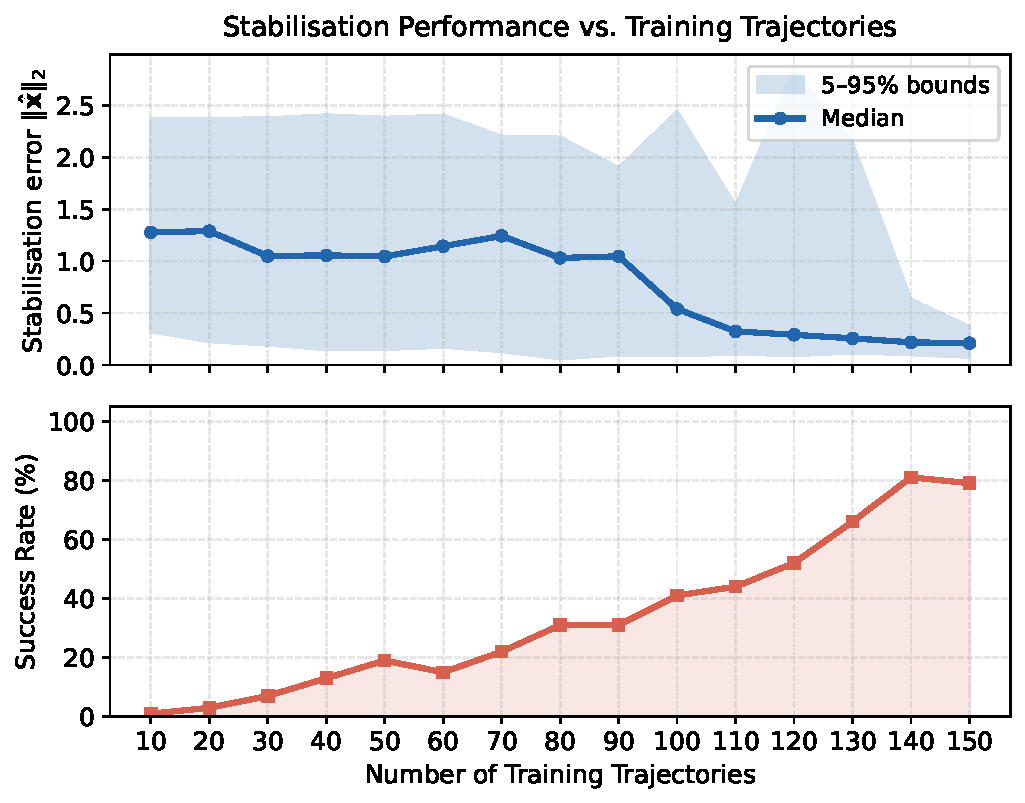
\includegraphics[width=\columnwidth]{figures/paper/fig1_stabilisation_performance.pdf}
  \caption{Stabilisation performance vs.\ training-set size (100 trials per
    point, mismatched plant).  \emph{Top:} median $e_{\mathrm{stab}}$
    (Eq.~\eqref{eq:estab}) with 5th--95th percentile band.
    \emph{Bottom:} paper-success rate (Eq.~\eqref{eq:success}).
    Both curves plateau near 150~demos; the main gain occurs between
    100--140~demos where the tail of the error distribution collapses.}
  \label{fig:fig1}
\end{figure}

Fig.~\ref{fig:fig1} reproduces the sweep experiment of Lee~\emph{et
al.}~\cite{lee2024} (their Fig.~3) using the hybrid observer.  At 40 demos the
success rate is only 13\%, compared to 97\% in the original paper.  This gap
arises directly from the structural difference in Table~\ref{tab:compare}: the
full observer of \cite{lee2024} learns non-zero $\Lmat$ rows for \emph{all four
states} from pixels, correcting $x$, $\dot x$, and $\dot\theta$ as well as
$\theta$.  The hybrid observer corrects only $\theta$, so it requires far more
data to achieve stable cart regulation through the LQR feedback loop.  By
140--150~demos, the angle regressor is accurate enough that the model-predicted
$x$ error remains within the controller's tolerance.

\subsection{Single-Rollout Time Histories}

\begin{figure*}[t]
  \centering
  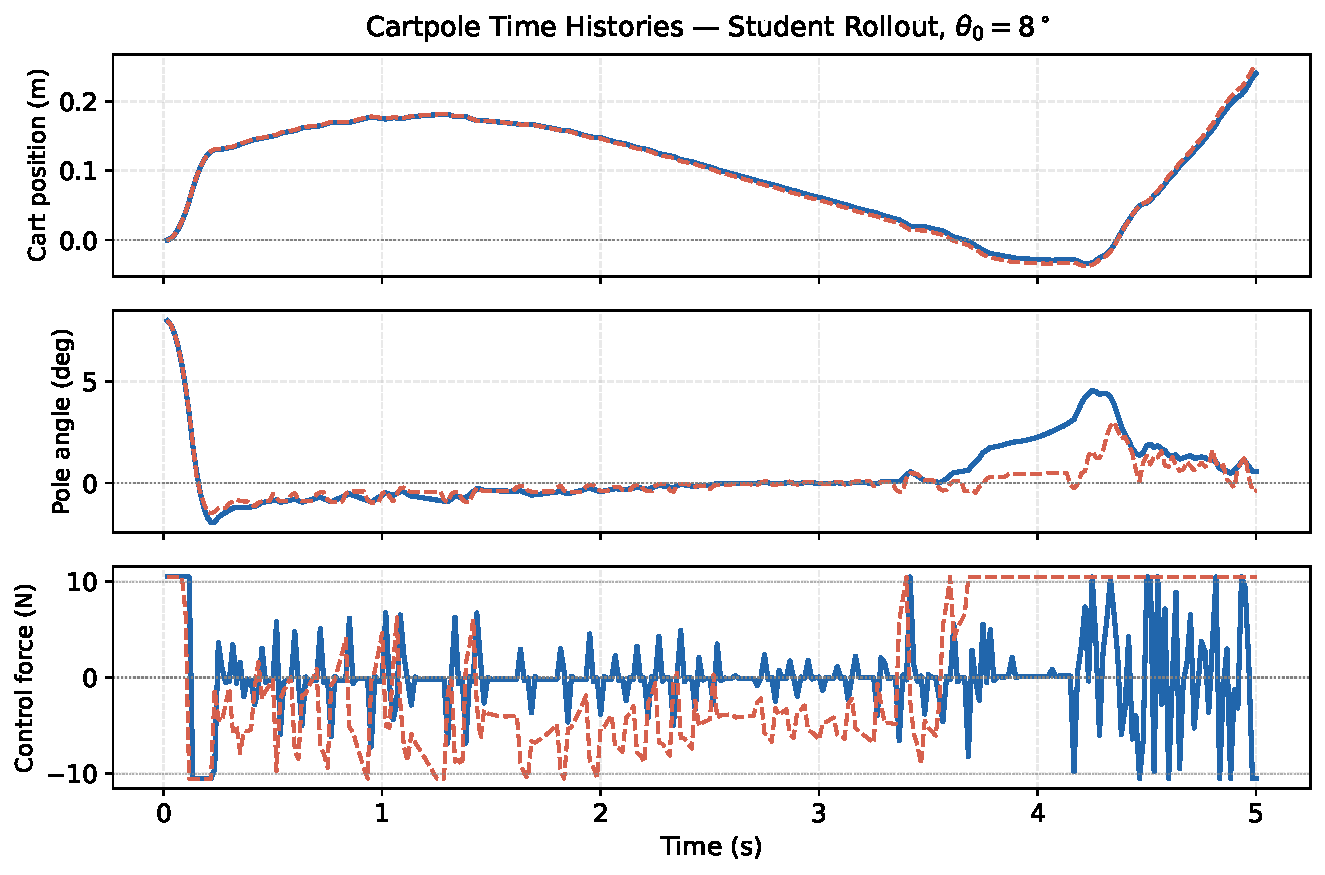
\includegraphics[width=\textwidth,height=0.45\textheight,keepaspectratio]{figures/paper/fig3_time_histories.pdf}
  \caption{Time histories for a single rollout at $\theta_0=8^\circ$
    (150-demo observer, mismatched plant).
    \emph{Top:} cart position; \emph{Middle:} pole angle.
    True state (solid) vs.\ observer estimate (dashed).
    \emph{Bottom:} applied control force vs.\ teacher anticipated command.
    The pole angle is tracked closely; cart position error accumulates but
    remains within the LQR basin.}
  \label{fig:fig3}
\end{figure*}

Fig.~\ref{fig:fig3} corresponds to Fig.~5b of Lee~\emph{et al.}~\cite{lee2024}
for a single stabilisation rollout.  The pole angle estimate (middle panel)
tracks the true angle tightly, while the cart position estimate (top panel)
drifts because only the open-loop model propagates $x$.  Despite this
estimation error, the applied control force (bottom panel) closely follows the
teacher-anticipated command, confirming that angle correction alone is
sufficient for closed-loop stabilisation within the 2.5~s window.

\subsection{Effective Gain and Spatial Interpretation}

The effective gain $\Lmat_{\mathrm{eff}}$ defined by \eqref{eq:Leff} has
non-zero entries only in its third row (pole angle).  These coefficients, when
reshaped to the frame geometry, concentrate near the pole tip---consistent with
the interpretable sparse structure reported in \cite{lee2024} (their Fig.~4,
$\theta$ row).  In contrast, \cite{lee2024} also reports non-zero cart and
velocity rows (Fig.~4a, 4b, 4d), which the fixed $\Lmat=\bm{0}$ structure of
the hybrid observer cannot reproduce.

\subsection{Quantitative Summary}

\begin{table}[t]
  \centering
  \caption{Observer Performance at 150 Training Demos\\
    (100 Evaluation Trials, Mismatched Plant)}
  \label{tab:results}
  \renewcommand{\arraystretch}{1.15}
  \begin{tabular}{lcc}
    \toprule
    Metric & This work & Lee et al.~\cite{lee2024} \\
    \midrule
    Training demos for success & 150   & 40--80    \\
    Student survival (150 demos) & 100\% & 100\%   \\
    Paper success (150 demos)    & 79\%  & $\ge$97\% \\
    $e_{\mathrm{stab}}$ median   & 0.210 & ---       \\
    $e_{\mathrm{stab}}$ 95th pct & 0.372 & ---       \\
    Ridge $R^2$ ($\theta$)       & 0.986 & ---       \\
    Ridge RMSE ($\theta$)        & $0.115^\circ$ & --- \\
    \bottomrule
  \end{tabular}
\end{table}

% ─────────────────────────────────────────────────────────────────────────────
\section{Conclusions}
\label{sec:conclusions}

\begin{enumerate}

  \item \textbf{The pixels-to-torques framework is reproducible with
    lightweight tools.}
    A Ridge regression model trained on raw binary frames replicates the
    angle-estimation accuracy ($R^2>0.98$, RMSE~$<0.12^\circ$) reported
    by Lee~\emph{et al.}~\cite{lee2024} without requiring a full LLS solve
    or stability-constrained optimisation.

  \item \textbf{Correcting only $\theta$ requires substantially more data.}
    At 40 demos, the success rate is 13\% versus 97\% in \cite{lee2024}.
    The full joint LLS observer learns pixel corrections for all four states
    simultaneously, giving it far better data efficiency because cart and
    velocity errors are damped directly rather than only indirectly through
    the LQR loop.

  \item \textbf{Cart-position estimation is the key open problem.}
    With no direct pixel signal for $x$ or the velocities, drift accumulates
    beyond the 2.5~s evaluation window.  Adding a second Ridge regressor for
    $x$ (feasible given that the pole-tip column encodes $x$, as in
    \eqref{eq:geometry}) is the natural next step toward matching
    full-observer performance.

  \item \textbf{The method is interpretable and connects to classical theory.}
    The effective gain \eqref{eq:Leff} makes the hybrid observer a special
    case of \eqref{eq:obs_lee}, enabling the same closed-loop stability
    analysis used in \cite{lee2024}.  The sparse, spatially localised pixel
    coefficients confirm the physical interpretation: the observer learns to
    look where the geometry says it should.

\end{enumerate}

% ─────────────────────────────────────────────────────────────────────────────
\IEEEtriggeratref{3}
\begin{thebibliography}{9}

\bibitem{lee2024}
J. H. Lee, S. Schoedel, A. Bhardwaj, and Z. Manchester,
``From pixels to torques with linear feedback,''
\emph{arXiv preprint arXiv:2406.18699v3}, Dec.\ 2024.

\bibitem{brockman2016openai}
G. Brockman \emph{et al.},
``OpenAI Gym,''
\emph{arXiv preprint arXiv:1606.01540}, 2016.

\bibitem{andrychowicz2020learning}
M. Andrychowicz \emph{et al.},
``Learning dexterous in-hand manipulation,''
\emph{Int.\ J.\ Robot.\ Res.}, vol.~39, no.~1, pp.~3--20, Jan.\ 2020.

\bibitem{levine2016end}
S. Levine, C. Finn, T. Darrell, and P. Abbeel,
``End-to-end training of deep visuomotor policies,''
\emph{J.\ Mach.\ Learn.\ Res.}, vol.~17, no.~1, pp.~1334--1373, 2016.

\bibitem{luenberger1964}
D. G. Luenberger,
``Observing the state of a linear system,''
\emph{IEEE Trans.\ Mil.\ Electron.}, vol.~8, no.~2, pp.~74--80, Apr.\ 1964.

\end{thebibliography}

\end{document}
